\documentclass{article}

% Language setting
% Replace `english' with e.g. `italian' to change the document language
\usepackage[english]{babel}

% Set page size and margins
% Replace `letterpaper' with `a4paper' for UK/EU standard size
\usepackage[letterpaper,top=2cm,bottom=2cm,left=3cm,right=3cm,marginparwidth=2cm]{geometry}

% Useful packages
\usepackage{tikz}
\usepackage{amsmath}
\usepackage{graphicx}
\usepackage{algorithm}
\usepackage{algpseudocode}
\usepackage[colorlinks=true, allcolors=blue]{hyperref}

\usetikzlibrary{shapes,arrows,positioning,calc}

\newcounter{example}[section]
\newenvironment{example}[1][]{\refstepcounter{example}\par\medskip
   \noindent \textbf{Example~\theexample. #1} \rmfamily}{\medskip}

\newcounter{definition}[section]
\newenvironment{definition}[1][]{\refstepcounter{definition}\par\medskip
   \noindent \textbf{Definition~\thedefinition. #1} \rmfamily}{\medskip}

\newcounter{fact}[section]
\newenvironment{fact}[1][]{\refstepcounter{fact}\par\medskip
   \noindent \textbf{Fact~\thefact. #1} \rmfamily}{\medskip}

\title{Public Key Cryptography}
\author{Federico Casu}

\begin{document}
\maketitle

\tikzset{
  block/.style = {draw, rectangle, text width=2.5cm, align=center, minimum height=1.5cm},
  arrow/.style = {thick,->,>=stealth},
  line/.style = {thick,-},
}

%%%%%%%%%%%%%%%%%%%%%%%%%%%%%%%%%%%%%%%%%%%%%%%%%%%%%%%%%%%%%%%%%%%%%%%%%%%%%%%%%%%%%%%%%%%%%%%%%%%%%%%%%%%%%%%%%%%%%%%%%%%%%
\section{Introduction}
As we are becoming familiar with it, let's delve into the application of $\mathsf{public}$ $\mathsf{key}$ $\mathsf{cryptography}$ in securing communications. Figure \ref{fig:pub_key_scenario} illustrates the fundamentals of a public key-based communication system:

\begin{enumerate}
    \item Alice, who wants to send a confidential message to Bob, knows Bob's public key $\mathsf{K_{pub}^{B}}$. To encrypt the message $\mathsf{x}$, Alice executes the encryption algorithm $\mathsf{E(\cdot)}$, taking as input the plaintext $\mathsf{x}$ and Bob's public key $\mathsf{K_{pub}^{B}}$.
    \item Bob, who wants to read the incoming message, executes the decryption algorithm $\mathsf{E^{-1}(\cdot)}$, taking as input the ciphertext $\mathsf{y}$ and Bob's private key $\mathsf{K_{priv}^{B}}$.
\end{enumerate}

\begin{figure}
    \centering
    \begin{tikzpicture}[node distance=3cm]

        % Alice
        \node [block] (Alice) {Alice knows $\mathsf{K_{pub}^{B}}$};

        % Bob
        \node [block, right=of Alice] (Bob) {Bob holds $\mathsf{\langle K_{priv}^{B}, K_{pub}^{B}\rangle}$};

        % Encryption and Decryption blocks
        \node [block, below=of Alice, yshift=1cm] (encrypt) {$\mathsf{y = E(K_{pub}^{B}, x)}$};
        \node [block, below=of Bob, yshift=1cm] (decrypt) {$\mathsf{x = E^{-1}(K_{priv}^{B}, y)}$};

        % Messages
        \node [below=0.25cm of encrypt] {$\mathsf{y}$: Encrypted Message};
        \node [below=0.25cm of decrypt] {$\mathsf{x}$: Original Message};

        % Arrows
        \draw [arrow] (Alice) -- node[above, xshift=0.75cm, yshift=-0.25cm] {$\mathsf{x \text{, } K_{pub}^{(B)}}$} (encrypt);
        \draw [arrow] (encrypt) -- node[left, xshift=1.45cm, yshift=0.25cm] {Insecure Channel} (decrypt);
        \draw [arrow] (Bob) -- node[above, xshift=0.75cm, yshift=-0.25cm] {$\mathsf{K_{priv}^{(B)}}$} (decrypt);

    \end{tikzpicture}
    \caption{Public Key Cryptography - Simple communication scenario.}
    \label{fig:pub_key_scenario}
\end{figure}

\par \noindent Let's establish a formal definition of a public key encryption scheme: a $\mathsf{public}$ $\mathsf{key}$ $\mathsf{encryption}$ $\mathsf{scheme}$ is a triple of algorithms, $\mathsf{\langle E, D, G\rangle}$, such that they fulfill the following properties:

\begin{enumerate}
    \item $\mathsf{G}$ is a randomized algorithm that outputs a pair of keys, namely $\mathsf{\langle K_{pub}, K_{priv} \rangle}$.
    $$
        \mathsf{G \text{ } : \text{ } \{0,1\}^{k} \rightarrow K = \{0,1\}^{n} \times \{0,1\}^{n}}
    $$
    \item $\mathsf{E}$ is a randomized algorithm that, given inputs of a plaintext $\mathsf{x \in M}$ and a public key $\mathsf{K_{pub}}$, outputs a ciphertext $\mathsf{y \in C}$.
    $$
    \mathsf{E \text{ } : \text{ } K \times M \rightarrow C}
    $$
    \item $\mathsf{D}$ is a \textbf{deterministic} algorithm that, given inputs of a ciphertext $\mathsf{y \in C}$ and a private key $\mathsf{K_{priv}}$, outputs a plaintext $\mathsf{x \in M}$.
    $$
    \mathsf{D \text{ } : \text{ } K \times C \rightarrow M}
    $$
    \item The encryption scheme fulfills the \textbf{consistency property}, \textit{i.e.}
    $$
        \mathsf{\forall \text{ } \langle K_{pub}, K_{priv} \rangle \text{, } \forall \text{ } x \in M \rightarrow E^{-1}(K_{priv}, E(K_{pub}, x)) = x}
    $$
\end{enumerate}

\par \noindent Being an encryption scheme means provide some security properties. We would like to give you an informal definition of the security properties of a public key encryption scheme:

\begin{enumerate}
    \item Given any ciphertext $\mathsf{y}$ and the public key used to encrypt it, $\mathsf{K_{\text{pub}}}$, it must be infeasible to obtain the plaintext $\mathsf{x}$ such that $\mathsf{y = E(K_{\text{pub}}, x)}$.
    \item Given any public key, it must be infeasible to obtain the corresponding private key.
\end{enumerate}
 
\par \noindent Such properties rely on some algebraic constructs. In particular, public key cryptography exploits a certain type of mathematical functions called \textbf{one-way} functions. The \textit{one-wayness} property states that a function $\mathsf{f}$ is said to be one-way if:

\begin{enumerate}
    \item $\mathsf{f \text{ } is \text{ } easy \text{ } to \text{ } compute}$
    \item $\mathsf{f^{-1} \text{ } is \text{ } hard \text{ } to \text{ } compute}$
\end{enumerate}

\par \noindent In what way $\mathsf{one\text{-}way}$ functions are related to public key cryptography? Let's make an example.

\begin{example}
    The $\mathsf{RSA}$ cryptosystem exploits the integer factorization as the underlying $\mathsf{one\text{-}way}$ function: multiplying two primes is easy but factoring the resulting product is computationally infeasible. $\mathsf{RSA}$ key generation algorithm security rely on the integer factorization problem.
\end{example}

\par \noindent Public key cryptography is not \textit{perfect}. Let's prove it:

\begin{enumerate}
    \item Let's consider that an attacker managed to obtain a ciphertext $\mathsf{y}$. 
    \item Let's consider a plaintext $\mathsf{\hat{x} \text{ } \in M}$ such that $\mathsf{0 < P(X = x) < 1}$. Knowing the receiver's public key (by definition, as the name suggests, is public), we encrypt the choosen plaintext $\mathsf{\hat{x}}$ with the public key, \textit{i.e.}, $\mathsf{\hat{y} = E(K_{pub}, \hat{x})}$. Now we are in front of two scenarios:
    \begin{enumerate}
        \item $\mathsf{y = \hat{y} \rightarrow x = \hat{x} \rightarrow P(X = \hat{x} \text{ } | \text{ } Y = y) = 1 \neq P(X = x)}$
        \item $\mathsf{y \neq \hat{y} \rightarrow x \neq \hat{x} \rightarrow P(X = \hat{x} \text{ } | \text{ } Y = y) = 0 \neq P(X = x)}$
    \end{enumerate}
\end{enumerate}

A public key encryption scheme is \textit{not} perfect because it's always possible to find a plaintext whose a-posteriori probability is either $\mathsf{0}$ or $\mathsf{1}$, which is different from $\mathsf{P(X=x)}$. \newline

\par \noindent Let's explore some real-world applications of public key cryptography:

\begin{enumerate}
    \item The first application is in digital communications. The primary distinction between a symmetric key encryption scheme and a public key encryption scheme is that the former requires an initial phase during which the communicating parties securely agree on the key used for encryption. In a public key encryption scheme, there is no need to securely agree on a session key. The encryption phase utilizes the public key, and the decryption phase uses the private key. Importantly, even if the public key is publicly known, the private key does not need to be transmitted over an insecure channel: only the owner can decrypt any messagge encrypted with the corresponding public key.
    \item Moving forward, we will delve into the study of digital signatures. The asymmetric nature of the encryption scheme makes public key cryptography more suitable for digital signature schemes compared to symmetric ones.
\end{enumerate}

\begin{figure}
    \centering
    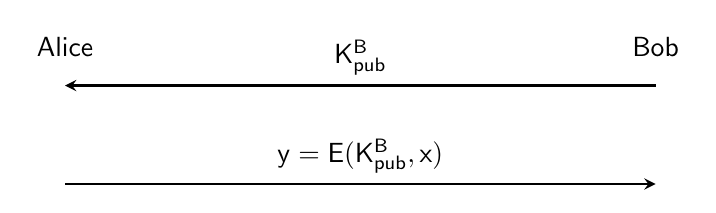
\begin{tikzpicture}[node distance=3cm, block/.style={draw, fill=blue!20, text width=2.5cm, text centered, rounded corners, minimum height=1.2cm},
    arrow/.style={thick, ->, >=stealth}]

        % Alice
        \coordinate (Alice) at (0,0);

        % Bob
        \coordinate (Bob) at (7.5,0);

        \node [above=0.25cm of Alice] {$\mathsf{Alice}$};
        \node [above=0.25cm of Bob] {$\mathsf{Bob}$};

        \coordinate (Alice_encrypt) at (0,-1.25);
        \coordinate (Bob_decrypt) at (7.5,-1.25);

        % Arrows
        \draw [arrow] (Bob) -- node[above] {$\mathsf{K_{pub}^{B}}$} (Alice);
        \draw [arrow] (Alice_encrypt) -- node[above] {$\mathsf{y = E(K_{pub}^{B}, x)}$} (Bob_decrypt);

    \end{tikzpicture}
    \caption{Simple $\mathsf{P}$ublic $\mathsf{K}$ey $\mathsf{E}$ncryption ($\mathsf{PKE}$) scheme.}
    \label{fig:pke_scheme}
\end{figure}

\par \noindent Public key encryption schemes have a big problem: public key encryption is $\mathsf{2\text{-}3}$ orders of magnitude slower than symmetric key encryption! A very simple communication scheme based on public key cryptography (Figure \ref{fig:pke_scheme}) cannot not be used in practice. A solution to this problem is given by the $\mathsf{digital}$ $\mathsf{envelope}$: public key cryptography is used only to encrypt the symmetric key (Figure \ref{fig:digital_envelope_scheme}). \newline

\begin{figure}
    \centering
    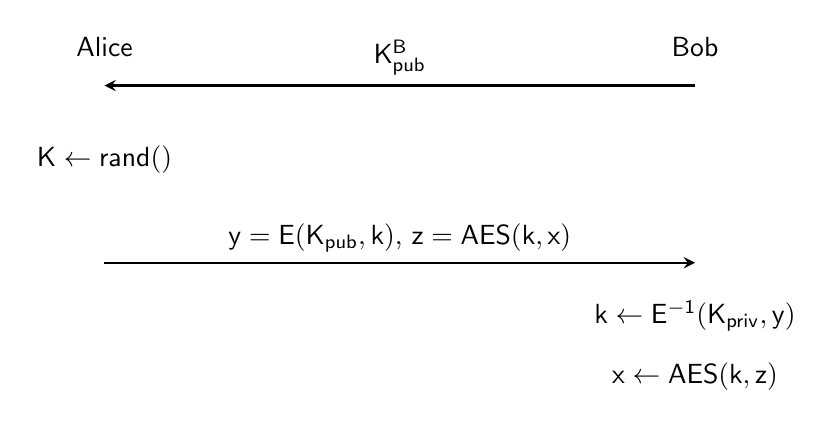
\begin{tikzpicture}[node distance=3cm, block/.style={draw, fill=blue!20, text width=2.5cm, text centered, rounded corners, minimum height=1.2cm},
    arrow/.style={thick, ->, >=stealth}]

        % Alice
        \coordinate (Alice) at (0,0);
        \node [above=0.25cm of Alice] {$\mathsf{Alice}$};

        % Bob
        \coordinate (Bob) at (7.5,0);
        \node [above=0.25cm of Bob] {$\mathsf{Bob}$};

        \coordinate (Alice_encrypt) at (0,-1.25);
        \node [above=0.005cm of Alice_encrypt] {$\mathsf{K \leftarrow rand()}$};

        \coordinate (Alice_send) at (0,-2.25);
        \coordinate (Bob_recv) at (7.5,-2.25);

        \coordinate (Bob_decrypt_K) at (7.5,-3.25);
        \node [above=0.005cm of Bob_decrypt_K] {$\mathsf{k \leftarrow E^{-1}(K_{priv}, y)}$};

        \coordinate (Bob_decrypt_z) at (7.5,-4);
        \node [above=0.005cm of Bob_decrypt_z] {$\mathsf{x \leftarrow AES(k, z)}$};

        % Arrows
        \draw [arrow] (Bob) -- node[above] {$\mathsf{K_{pub}^{B}}$} (Alice);
        \draw [arrow] (Alice_send) -- node[above] {$\mathsf{y = E(K_{pub}, k) \text{, } z = AES(k, x)}$} (Bob_recv);

    \end{tikzpicture}
    \caption{Digital Envelope communication protocol.}
    \label{fig:digital_envelope_scheme}
\end{figure}

\par \noindent What about the \textit{security level} of a public key encryption scheme? The formal definition of security level is the following:

\begin{definition}
    An encryption scheme has $\mathsf{security}$ $\mathsf{level}$ of $\mathsf{n}$ bits if the best known algorithm to break it requires $\mathsf{2^n}$ steps.
\end{definition}

\par \noindent The relationships between the key length and the security level in a symmetric encryption scheme is straightforward: if the key is $\mathsf{n}$ bits long then the encryption scheme has security level of $\mathsf{n}$ bits. For public key encryption schemes is a bit different: there is no linear relation between key lenght and security level: as a rule of thumb, the computational complexity grows roughly with the cube bit length.

\begin{figure}
    \centering
    \includegraphics[width=0.75\linewidth]{figures/security_level.png}
    \caption{\label{fig:security_level}Security level of the most used encryption schemes.}
\end{figure}


\subsection{Key Authentication: MITM Attacks}

With respect to a passive attacker, any public key encryption scheme is secure. If an attacker intercepts any ciphertext, they must solve the underlying mathematical problem to be able to decrypt the intercepted cyphertext. Therefore, if the encryption scheme is well-designed (meaning that the encryption scheme exploits a good \textit{one-way} function), the attacker will not be able to decrypt or obtain the private key in a reasonable amount of time. \newline

\par \noindent Now, considering an active attacker, let's explore the following scenario (Figure \ref{fig:mitm}):

\begin{enumerate}
    \item Oscar is a "bad guy" who wishes to secretly read the messages that Alice and Bob are going to exchange.
    \item Bob needs to let Alice know his current public key: he simply sends his public key through an insecure channel. Bob doesn't worry about the public key and he thinks that Alice correctly receives  his public key.
    \item Oscar manages to intercept Bob's public key. He's a smart guy and he thinks to impersonate Bob by sending to Alice a freshly generated public key $\mathsf{K_{pub}^{O}}$.
    \item Alice receives Oscar's public key but she thinks that it was Bob who sent the message. So she encrypts the confidential message with the received public key and sends it through the insecure channel.
    \item Oscar, once again, intercepts the encrypted message. Since the latter was encrypted using his public key, he is able to correctly decrypt Alice's message, read $\mathsf{x}$ and send $\mathsf{c' = E(K_{pub}^{B}, x)}$ to Bob.
    \item Bob receives Oscar's messagge thinking that it was sent by Alice: both Alice and Bob are scammed by Oscar and no one knows it!
\end{enumerate}

\begin{figure}
    \centering
    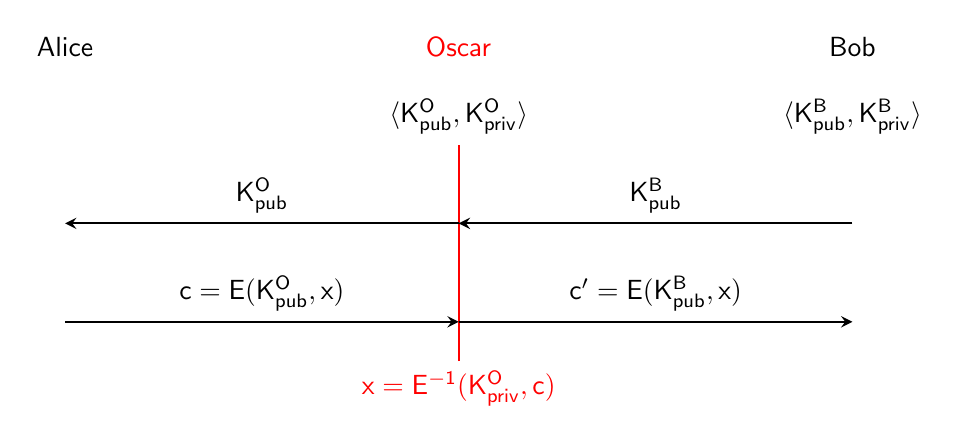
\begin{tikzpicture}[node distance=3cm, block/.style={draw, fill=blue!20, text width=2.5cm, text centered, rounded corners, minimum height=1.2cm},
    arrow/.style={thick, ->, >=stealth}]

        % Alice
        \coordinate (Alice) at (0,0);

        % Oscar (the attacker)
        \coordinate (Oscar) at (5,0);
        \draw[red, thick] ($(Oscar) + (0,-3.5)$) -- ($(Oscar) + (0,-0.75)$);


        % Bob
        \coordinate (Bob) at (10,0);

        \node [above=0.25cm of Alice] {$\mathsf{Alice}$};
        \node [above=0.25cm of Oscar] {\textcolor{red}{$\mathsf{Oscar}$}};
        \node [below=0.05cm of Oscar] {$\mathsf{\langle K_{pub}^{O}, K_{priv}^{O} \rangle}$};
        \node [below=3.50cm of Oscar] {\textcolor{red}{$\mathsf{x = E^{-1}(K_{priv}^{O}, c)}$}}; 
        \node [above=0.25cm of Bob] {$\mathsf{Bob}$};
        \node [below=0.05cm of Bob] {$\mathsf{\langle K_{pub}^{B}, K_{priv}^{B} \rangle}$};

        \coordinate (Alice_recv_pk) at (0,-1.75);
        \coordinate (Oscar_substitute_pk) at (5,-1.75);
        \coordinate (Bob_send_pk) at (10,-1.75);

        \coordinate (Alice_send_c) at (0,-3);
        \coordinate (Oscar_substitute_c) at (5,-3);
        \coordinate (Bob_recv_c) at (10,-3);

        % Arrows
        \draw [arrow] (Bob_send_pk) -- node[above] {$\mathsf{K_{pub}^{B}}$} (Oscar_substitute_pk);
        \draw [arrow] (Oscar_substitute_pk) -- node[above] {$\mathsf{K_{pub}^{O}}$} (Alice_recv_pk);

        \draw [arrow] (Alice_send_c) -- node[above] {$\mathsf{c = E(K_{pub}^{O}, x)}$} (Oscar_substitute_c);
        \draw [arrow] (Oscar_substitute_c) -- node[above] {$\mathsf{c' = E(K_{pub}^{B}, x)}$} (Bob_recv_c);

    \end{tikzpicture}
    \caption{$\mathsf{M}$an $\mathsf{I}$n $\mathsf{T}$he $\mathsf{M}$iddle ($\mathsf{MITM}$) attack.}
    \label{fig:mitm}
\end{figure}

\par \noindent How can we prevent a \textit{man-in-the-middle} attack? Let's study a possible solution:

\begin{example}
    Instead of sending their own public key, each user registers their public key with a \textit{trusted read-only repository}. Whenever Alice wants to send a confidential message to Bob, she queries the trusted repository, asking for Bob's public key.
\end{example}

\par \noindent Note that a trusted repository does not secure a public encryption scheme from MITM attacks: an adversary could intercept the query for a public key and craft a fake response substituting the legit public key with any key they want. Later on, we will study how public key encryption schemes exploit digital signatures to mitigate MITM attacks.


\subsection{Encryption Randomization}

There are some scenarios that require to be studied because a plain public key encryption scheme is vulnerable. Let's examine it:

\begin{enumerate}
    \item Consider an auction. Alice, a bidder participating in Bob's auction, sends her bid to Bob by encrypting it with Bob's public key.
    \item Oscar, a bad guy, wishes to win the auction by spending the least amount of money possible. He does this by sending a bid with an amount equal to the maximum bid from honest bidders plus 1 dollar. Since Oscar knows the market value of the goods being auctioned, he knows that the bids can be represented with 10 bits, meaning each bid is 10 bits long.
    \item Oscar manages to obtain each bid sent to Bob. Since Oscar knows Bob's public key (if Oscar couldn't obtain Bob's public key, then the latter would be a private key!), he performs the attack described in Algorithm \ref{alg:small_plaintext_attack}.
    \item The attack complexity is very low: $\mathsf{O(2^{10})}$. Oscar can brute-force each intercepted message (perhaps in parallel) and obtain the highest bid that was sent to Bob. Once he has done that, he can device all the participants by sending to Bob $\mathsf{y = E(K_{pub}^{B}, \text{max} + 1)}$.
\end{enumerate}

\begin{algorithm}
    \caption{Small plaintext attack: algorithm}
    \label{alg:small_plaintext_attack}
    \begin{algorithmic}
        \For{$\mathsf{i \gets 0 \text{ } to \text{ } 2^{10}}$}
            \State $\mathsf{y' \gets \text{ } encrypt(K_{pub}, i)}$
            \If{$\mathsf{y = y'}$}
                \Return $\mathsf{i}$
            \EndIf
        \EndFor
    \end{algorithmic}
\end{algorithm}

Is there a way to prevent Bob and the bidders from being scammed? Yes:

\begin{enumerate}
    \item Each bidder generates a random number $\mathsf{g \text{ } \in \text{ } \{0,1\}^{r}}$.
    \item Now, instead of encrypting only the bid, the message to be encrypted is the following:
    $$
        \mathsf{x' = x \text{ } | \text{ } g}
    $$
    \item Oscar, to obtain the bid $\mathsf{x}$ from the encrypted message, needs to executes Algorithm \ref{alg:small_plaintext_attack_salt}.
    \item The attack's complexity gets multiplied by $\mathsf{2^r}$!
\end{enumerate}

\begin{algorithm}
    \caption{Small plaintext attack: algorithm}
    \label{alg:small_plaintext_attack_salt}
    \begin{algorithmic}
        \For{$\mathsf{i \gets 0 \text{ } to \text{ } 2^{10}}$}
            \For{$\mathsf{j \gets 0 \text{ } to \text{ } 2^{r}}$}
                \State $\mathsf{y' \gets \text{ } encrypt(K_{pub}, \{i, j\})}$
                \If{$\mathsf{y = y'}$}
                    \Return $\mathsf{i}$
                \EndIf
            \EndFor
        \EndFor
    \end{algorithmic}
\end{algorithm}
%%%%%%%%%%%%%%%%%%%%%%%%%%%%%%%%%%%%%%%%%%%%%%%%%%%%%%%%%%%%%%%%%%%%%%%%%%%%%%%%%%%%%%%%%%%%%%%%%%%%%%%%%%%%%%%%%%%%%%%%%%%%%
\newpage
%%%%%%%%%%%%%%%%%%%%%%%%%%%%%%%%%%%%%%%%%%%%%%%%%%%%%%%%%%%%%%%%%%%%%%%%%%%%%%%%%%%%%%%%%%%%%%%%%%%%%%%%%%%%%%%%%%%%%%%%%%%%%
\section{RSA Cryptosystem}

\par \noindent $\mathsf{RSA}$ cryptosystem was invented by a group of researchers (R. L. Rivest, A. Shamir and L. Adleman) working at MIT Laboratory for Computer Science. The encryption scheme was first presented in a paper called "A Method for Obtaining Digital Signatures and Public-Key Cryptosystems" (February $\mathsf{1978}$). Let's delve into the fundamentals of the RSA encryption scheme.

\paragraph{Key Generation Algorithm} Formally, the RSA key generation algorithm is composed by 5 steps:

\begin{algorithm}
\caption{RSA Key Generation Algorithm}
\label{alg:key_generation}
\begin{algorithmic}[1]
    \State Choose two large prime numbers, namely $\mathsf{p}$ and $\mathsf{q}$.
    \State Compute the quantity $\mathsf{n = p \cdot q}$ called \textit{modulus}.
    \State Compute the quantity $\mathsf{\phi = (p-1)(q-1)}$.
    \State Choose $\mathsf{e}$ such that $\mathsf{1 < e < \phi}$ and $\mathsf{gcd(e, \phi) = 1}$.
    \State Choose $\mathsf{d}$ such that $\mathsf{1 < d  < \phi}$ and $\mathsf{e \cdot d \equiv 1 \pmod{\phi}}$.
\end{algorithmic}
\end{algorithm}

\par \noindent The key generation algorithm outputs two quantities:
\begin{align*}
    \mathsf{public} \text{ } \mathsf{key} &: \mathsf{\langle e, n \rangle} \\
    \mathsf{private} \text{ } \mathsf{key} &: \mathsf{\langle d, n \rangle} 
\end{align*}

\paragraph{Encryption and Decryption Algorithm}
\begin{align*}
    \mathsf{Encryption} &: \mathsf{y = x^{e} \mod n} \\
    \mathsf{Decryption} &: \mathsf{x = y^{d} \mod n}
\end{align*}

\par \noindent Now we need to discuss the performance of the key generation algorithm. In particular, generating a pair of keys $\mathsf{\langle K_{pub}, K_{priv} \rangle}$ involves some operations:

\begin{enumerate}
    \item Find two large prime numbers. Obviously, each prime needs to be randomly generated (otherwise an attacker could guess the prime with a very high probability). 
    \item Test whether or not the randomly generated number is truly a prime number.
    \item Find a public and a private exponent which fulfill the required properties: $\mathsf{gcd(e, \phi) = 1}$ and $\mathsf{e \cdot d \equiv 1 \pmod{\phi}}$.
\end{enumerate}

\par \noindent So the prime generation algorithm could be pseudo coded as follows:

\begin{algorithm}
    \caption{Prime Generation Algorithm}
    \label{alg:prime_generator}
    \begin{algorithmic}
        \Repeat
            \State $\mathsf{p \gets random()}$
        \Until{$\mathsf{is\_prime(p) == False}$}
    \end{algorithmic}
\end{algorithm}

\par \noindent To establish the complexity of Algorithm \ref{alg:prime_generator} we need to answer the following questions:
\begin{enumerate}
    \item How many iterations do we need to execute? In other words, how likely is to find a prime $\mathsf{p < x}$?
    \item How difficult is it to generate a random number?
    \item How difficult is it to test whether a number is prime or not?
\end{enumerate}

\par \noindent Let's answer the previous questions:

\begin{fact}
    Let's call $\mathsf{\pi(x)}$ the number of primes which are $\mathsf{\leq x}$. If $\mathsf{x}$ is sufficiently big, then $\mathsf{\pi(x)}$ could be approximated to $\mathsf{\pi(x) = \frac{x}{ln(x)}}$.
\end{fact}

\par \noindent If we test only odd integers, meaning that we test half the numbers $\mathsf{\in \text{ } [1, x]}$, the probability to find a prime $\mathsf{p \in [1, x]}$ is:
$$
    \mathsf{P(p \text{ } is \text{ } prime) = \frac{\pi(x)}{number \text{ } of \text{ } odds \in [2,x]} = \frac{x/ln(x)}{x/2} = \frac{2}{ln(x)} = O \left( \frac{1}{ln(x)} \right)}
$$

\par \noindent So, the expected number of trials needed to find a prime is $\mathsf{O(ln(x))}$, which is quite good (and easy). What about the complexity of a primality test? Primality tests are computationally much easier than factorization. In particular, practical implementations of primality tests are \textit{probabilistic}: at the question "is $\mathsf{p*}$ prime?" they answer
\begin{enumerate}
    \item $\mathsf{p*}$ is composed which is always a true statement;
    \item $\mathsf{p*}$ is prime, which is only true with a high probability.
\end{enumerate}

\par \noindent Now we need to discuss how difficult is to find a pair of keys such that fulfill the properties:
\begin{align*}
    \mathsf{gcd(e, \phi) = 1} \\
    \mathsf{e \cdot d \equiv 1 \pmod{\phi}}
\end{align*}

%To find the public exponent $\mathsf{e}$
%%%%%%%%%%%%%%%%%%%%%%%%%%%%%%%%%%%%%%%%%%%%%%%%%%%%%%%%%%%%%%%%%%%%%%%%%%%%%%%%%%%%%%%%%%%%%%%%%%%%%%%%%%%%%%%%%%%%%%%%%%%%%



\end{document}
